\chapter{Implementation}

\section{Implementation}
- This section shows a implementation of a testing utility for Scratch
- Uses the approach described above
- Implemented in JavaScript for compatibility with Scratch 3.0, which is implemented in JavaScript

\begin{itemize}
    \item System design / Components
        \begin{itemize}
            \item Sprites
            \item Callbacks
            \item Inputs
            \item Constraints
        \end{itemize}
    \item The step loop
    \item Coverage measuring
        \begin{itemize}
            \item What kind blocks are measured
            \item How is coverage measured (only reachable blocks)
        \end{itemize}
\end{itemize}

\begin{figure}
    \centering
    \tikzset{>=latex,
             label/.style={draw=none, text width=5.3cm, minimum height=0.5cm, text centered},
               box/.style={draw,      text width=2.5cm, minimum height=0.7cm, text centered, rounded corners},
                 h/.style={fill=blue!10}}

    \begin{tikzpicture}
        \node[box]   at ( 0.0,  3.0) (testfw)        {Test Framework};
        \node[box]   at ( 0.0,  1.5) (testdriver)    {Test Driver};
        \node[label] at ( 0.0,  0.0) (vmwrapper)     {VM Wrapper};
        \node[box]   at (-1.4, -0.7) (sprites)       {Sprites};
        \node[box]   at (-1.4, -1.6) (inputs)        {Inputs};
        \node[box]   at ( 1.5, -0.7) (callbacks)     {Callbacks};
        \node[box]   at ( 1.5, -1.6) (constraints)   {Constraints};
        \node[box]   at (-2.0, -3.2) (scratchvm)     {Scratch VM};
        \node[box]   at ( 2.2, -3.2) (scratchrender) {Renderer};

        \begin{scope}[on background layer]
            \node[draw, h, rounded corners, fit=(vmwrapper)(sprites)(inputs)(callbacks)(constraints)] (container) {};
        \end{scope}

        \foreach \pp/\pf/\pt in {--/testfw/testdriver,
                                 --/testdriver/container,
                                 --/container/scratchvm,
                                 --/container/scratchrender,
                                 --/scratchvm/scratchrender}
        \draw[shorten >= 2pt, ->] (\pf) \pp (\pt);
    \end{tikzpicture}

    \caption{Components of Whisker}
    \label{fig:components_of_whisker}
\end{figure}

\begin{figure}
    \centering
    \tikzset{>=latex,
             box/.style={draw, text width=4.3cm, minimum height=0.7cm, text centered, rounded corners},
             num/.style={draw, circle, inner sep=0.6mm, text centered},
               h/.style={fill=blue!10}}

    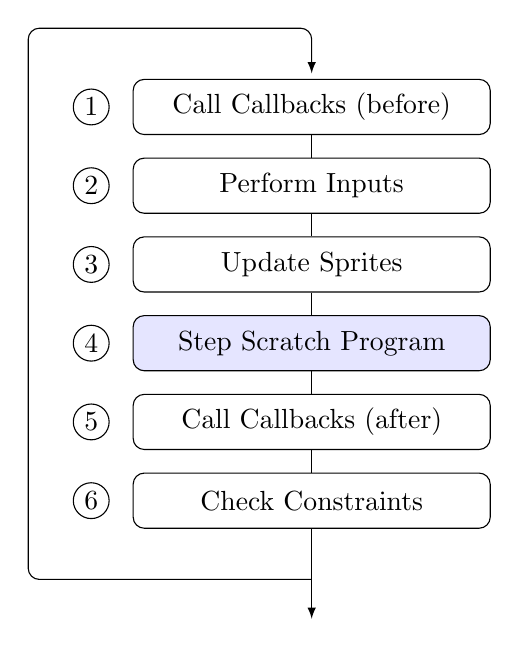
\begin{tikzpicture}
        \node[box]    at ( 0.2,  5.0) (callbacksbefore) {Call Callbacks (before)};
        \node[box]    at ( 0.2,  4.0) (inputs)          {Perform Inputs};
        \node[box]    at ( 0.2,  3.0) (sprites)         {Update Sprites};
        \node[box, h] at ( 0.2,  2.0) (step)            {Step Scratch Program};
        \node[box]    at ( 0.2,  1.0) (callbacksafter)  {Call Callbacks (after)};
        \node[box]    at ( 0.2,  0.0) (constraints)     {Check Constraints};

        \node[num] at (-2.6,  5.0) (one)   {1};
        \node[num] at (-2.6,  4.0) (two)   {2};
        \node[num] at (-2.6,  3.0) (three) {3};
        \node[num] at (-2.6,  2.0) (four)  {4};
        \node[num] at (-2.6,  1.0) (five)  {5};
        \node[num] at (-2.6,  0.0) (six)   {6};

        \draw[->]
            (callbacksbefore)
            -- (inputs)
            -- (sprites)
            -- (step)
            -- (callbacksafter)
            -- (constraints)
            -- ( 0.2, -1.5);

        \draw[shorten >= 2pt, rounded corners, ->]
            ( 0.2, -1.0)
            -- (-3.4, -1.0)
            -- (-3.4,  6.0)
            -- ( 0.2,  6.0)
            -- (callbacksbefore);
    \end{tikzpicture}

    \caption{Whisker Step Procedure}
    \label{fig:whisker_step_procedure}
\end{figure}

\begin{figure}
    \centering
    \begin{javascriptcode}
        STEP_TIME = 1000 / STEPS_PER_SECOND;
        WORK_TIME = 0.75 * STEP_TIME;

        while (running &&
               timeElapsed < WORK_TIME &&
               !redrawRequested) {
            for (thread of threads) {
                stepThread(thread);
            }
        }

        renderer.draw();
    \end{javascriptcode}
    \caption{Simplified Scratch Step Procedure}
    \label{fig:simplified_scratch_step_procedure}
\end{figure}

\section{Running Tests}
\label{sec:running_tests}
- Whisker comes with an optional testing framework
- Include a sample test report?

=== Seeing test output, interactive tests
- Users will want to see the program's output while it is run
    - to check if the tests run correctly, to check if the program runs correctly
    - Difficult to determine a problem with the project from just textual test reports
    - Tests without showing output are not very useful in such an interactive environment
$\rightarrow$ Has to be able to run in a interactive environment
    - Web GUI, which can be run by any modern browser
    - Allows users to run individual tests on the project and see the program execution

=== Batch Testing of Projects
- Some tests for Scratch projects can take a long time because projects run in real time
    - raises the need to test scratch programs in parallel
    - Scratch depends on the renderer
        - Some functionality of the Scratch virtual machine depends on the renderer
        - Headless tests are impossible without restricting the Scratch program to a subset of available blocks
$\rightarrow$ Web GUI has the option to run tests on multiple projects sequentially, but this might still take a long time depending on the project and the test suite
$\rightarrow$ Electron
    - Running tests in multiple processes could circumvent the problem
    - Electron provides a renderer that can be used to render the Scratch output to
    - Spawns multiple processes which open a window each, one project is tested in each window
